



\section{Obtaining a Gauss code for the link}

At this point, we have the link as a set of cyclic sequences of points in $\mathbb{R}^3$.
We also have the framing of each component. Thus the theoretical problem is solved. 
However, it is convenient to go on getting adequate planar projections to produce 
planar diagram for the link.
We obtain the following Gauss code, 
(\cite{rosenstiehl1976solution}, chapter 3 of \cite{Lins1980}, 
\cite{lins2008hsg}),
where signs mean
up $(+)$ and down $(-)$ passages:
$ ((-2,+3, -4,+1), (-5, +6, +2, -1),$ $(-3, +4, -7, -6, +5, +7)).$
From this code we get the link planar diagram of 
Figs. \ref{fig:r24_5link2}.
Since we have the framings curls
can be removed. An explicit elegant framed link inducing the euclidean 
3-manifold $|r^{24}_5|$ was previously unknown. We use 
Fig. \ref{fig:r24_5link} as input for L. Lins's software \cite{lins2007blink} to obtain
the WRT-invariants from $r=3$ to $r=20$ for the space $|r^{24}_5|$. We also apply our algorithm
for the Weber-Seifert hyperbolic dodecahedron space, obtaining a link with
142 crossings, included in Appendix B.

\begin{figure}[!htb]
\begin{center}
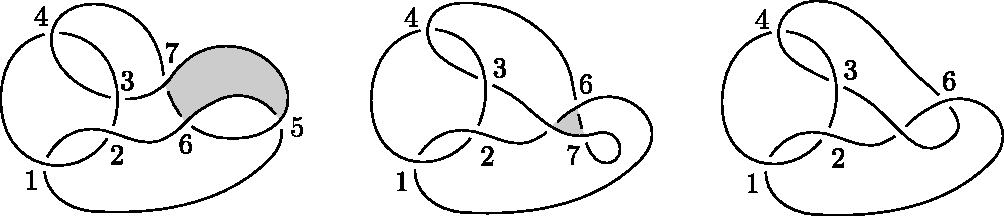
\includegraphics[width=12cm]{A.figs/r24_5link2.pdf}
\caption{Simplifying the link diagram for $|r_5^{24}|$.}
\label{fig:r24_5link2}
\end{center}
\end{figure}


\begin{figure}[!htb]
\begin{center}
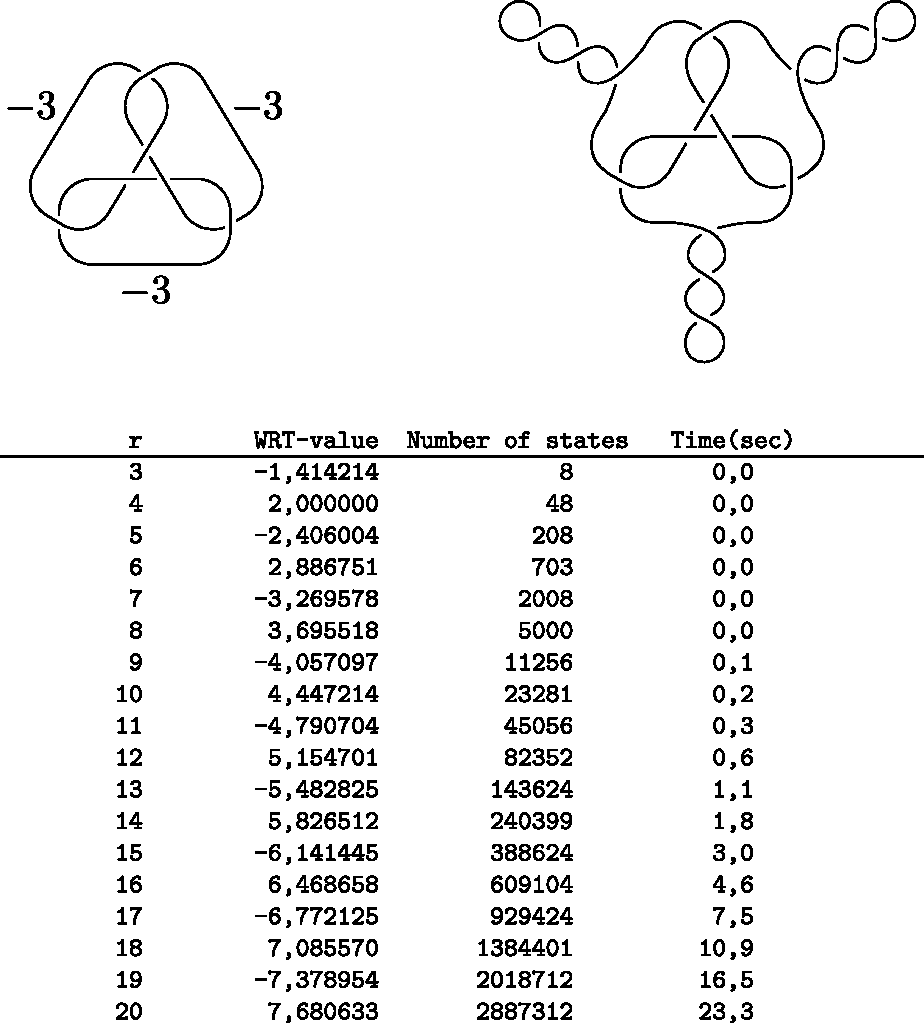
\includegraphics[width=11cm]{A.figs/r24_5link.pdf}
\caption{Framed link, blackboard framed link and WRT-invariants for $|r_5^{24}|$.
 %These invariants assume real values because the space is symmetric: the two
%oriented forms agree.
 Data obtained from L. Lins software \cite{lins2007blink}.}
\label{fig:r24_5link}
\end{center}
\end{figure}

%\begin{figure}[!htb]
%\begin{center}
%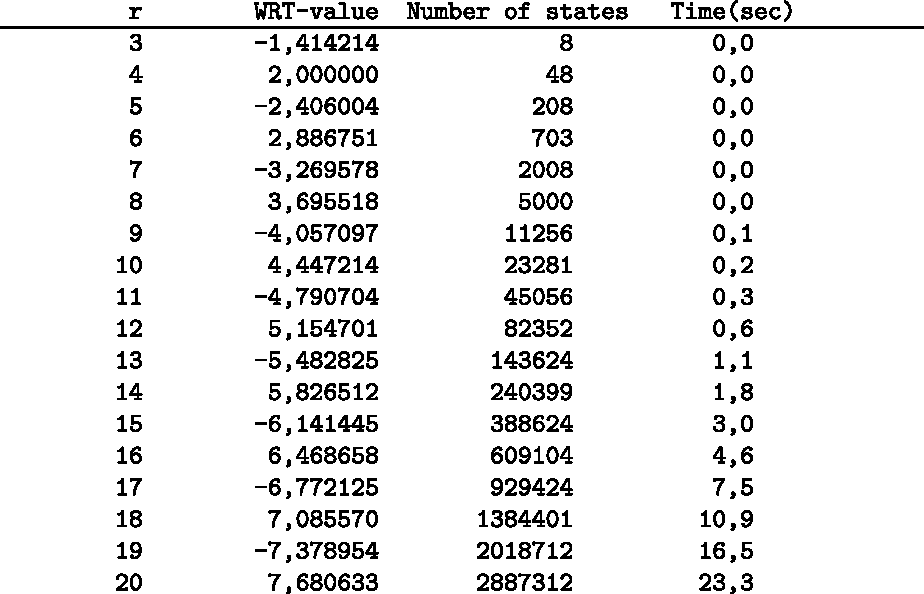
\includegraphics[width=13cm]{A.figs/r24_5linkinvariants.pdf}
%\caption{ WRT-invariants for $|r_5^{24}|$.
% These invariants assume real values because the space is symmetric: the two
%oriented forms agree. Data obtained from L. Lins software \cite{lins2007blink}.}
%\label{fig:r24_5link}
%\end{center}
%\end{figure}

\newpage
\begin{algorithm}
\label{theo:algorithm}
 There exists an $O(n^2)$-algorithm to produce, from a
  resoluble gem inducing an $M^3$,  a blackboard framed link also inducing $M^3$.
\end{algorithm}
\begin{proof} 
We start with a resoluble gem $G$ with $2n$ vertices. Here is the algorithm,
justified by the theory previously developed:
\begin{itemize}
 \item Form decreasing sequence of gems starting with $\mathcal{J}^2$,
 the $J^2$-gem associated with
the resolution of $G$ performing adequate $0$- or $1$-flips
 and finishing at the bloboid $\mathcal{B}_1$:
$\mathcal{J}^2=\mathcal{H}_{n},  \mathcal{H}_{n-1}, \ldots, \mathcal{H}_1=\mathcal{B}_1$.
%See Fig. \ref{fig:j2gemrSEQ} for the $r^{24}_5$-example.
 
 \item Form sequence of balloons $\mathcal{B}_1^\star,\ldots, \mathcal{B}_{n-1}^\star$
and pillows $\mathcal{P}_2^\star,\ldots, \mathcal{P}_n^\star$ defining implicitly the 
  sequence of combinatorial $2$-complexes $\mathcal{H}_1^\star, \mathcal{H}_1^\star, 
\ldots, \mathcal{H}_{2n}^\star$, together with 
their respective wings and nervures (combinatorially   
given by rotations), 
$\mathcal{W}_1^\ell \cup \mathcal{N}_1^\ell$, 
$\mathcal{W}_2^\ell \cup \mathcal{N}_2^\ell$,
\ldots, $\mathcal{W}_n^\ell \cup \mathcal{N}_n^\ell$ and 
$\mathcal{W}_1^r \cup \mathcal{N}_1^r$, 
$\mathcal{W}_2^r \cup \mathcal{N}_2^r$,
\ldots, $\mathcal{W}_n^r \cup \mathcal{N}_n^r$.
Each $bp$-move is simply a flip in the
primal sequence. See Figs. \ref{fig:winglist01} to \ref{fig:winglist11}
from the $r^{24}_5$-example.

\item Use Tutte's barycentric method with the edge weight 
heuristic (Fig. \ref{fig:arvorecompesos} from the $r^{24}_5$-example) 
to provide rectilinear embeddings
of $\mathcal{W}_n^\ell \cup \mathcal{N}_n^\ell$ in $\Pi_\ell$ and
of $\mathcal{W}_n^r \cup \mathcal{N}_n^r$ in $\Pi_r$ fixing the outer regions.
The nervures
are useful up to this point, and after obtaining the rectilinear embeddings
they can be discarded.

\item Get $\mathcal{H}_{1}^\diamond$ using
$\mathcal{W}_n^\ell \cup \mathcal{W}_n^r$ 
by the cone construction.


\item Get the sequence $\mathcal{H}_{2}^\diamond, \ldots, \mathcal{H}_{n}^\diamond = \mathcal{H}_n^\star$
by the blowing up technique in the proof of Theorem \ref{theo:teoremadeumalinha}.

\item Define the framings of the components of the link
as the linking numbers of the boundaries of the cylinders formed by
the strips coming from the hinges; special care: distinguish the
hinges which become 2-hinges from the
hinges which become 3-hinges in $M^3$. See Fig. \ref{fig:strips}.

\item Find an adequate projection of suitable medial curves in the cylinders.
These curves form the link. Find Gauss code for the link, and so,
a projection is combinatorially specified (\cite{rosenstiehl1976solution}, 
chapter 3 of \cite{Lins1980}, 
\cite{lins2008hsg}). Add curls to produce
a blackboard framed link. See Figs. \ref{fig:r24_5link2} and \ref{fig:r24_5link}
from the $r^{24}_5$-example.
\end{itemize}
This algorithm has both space complexity and time complexity $O(n^2)$.
Its output, first obtained as a set with no more than $n$ 
PL-polygons in $\mathbb{R}^3$,  
has a total of at most $12n^2$ vertices.
\end{proof}


%\chapter{Table of QI of spaces EUCLID$_i$}

%\section{EUCLID$_0$: Rep. $r_1^{24}$}

%\begin{figure}[!htb]
%\begin{center}
%\includegraphics[width=10.5cm]{A.figs/r24-1.pdf}
%\caption{3-gem, blackboard framed link for $|r_1^{24}|$ and
%WRT-invariants.}
%\label{fig:r24_5link}
%\end{center}
%\end{figure}

%\newpage

%\section{EUCLID$_1$: Rep. $r_5^{24}$}

%\begin{figure}[!htb]
%\begin{center}
%\includegraphics[width=10.5cm]{A.figs/r24_5GemLinkWRT.pdf}
%\caption{3-gem, blackboard framed link for $|r_5^{24}|$ and
%WRT-invariants.}
%\label{fig:r24_5link}
%\end{center}
%\end{figure}

%\newpage

%\section{EUCLID$_3$: Rep. $r_6^{24}$}%

%\begin{figure}[!htb]
%\begin{center}
%\includegraphics[width=10.5cm]{A.figs/r24_6.pdf}
%\caption{3-gem, blackboard framed link for $|r_6^{24}|$ and
%WRT-invariants.}
%\label{fig:r24_5link}
%\end{center}
%\end{figure}

%-----------------------------------

%\bibliographystyle{is-alpha}
%\addcontentsline{toc}{bibliografia}{\MakeTextUppercase{Refer�ncias Bibliogr�ficas}}
%\bibliography{d:/slsl\3.DadosSostenes.35.ArtigosLivros.bibtexGoogleScholar/bibtexIndex.bib} % bib file is slsl.bib
%\bibliography{~/home/ricardo/Dropbox/35.ArtigosLivros.bibtexGoogleScholar/bibtexIndex.bib}
%\bibliography{bibtexIndex.bib}
%\bibliography{slsl}

% \printindex
-----------


%\section{Appendix A: Proofs}\label{appA}

%\begin{proposition}
%\label{prop:planetwist}
%Let $G$ be a gem. $(a)$ A $ji$-twisting of a $j$-twistor of $G$ is factorable as
%one $i$-flip and one $j$-flip.
%$(b)$ If $G$ has a $0$-consecutive labelling on its vertices,
%then a $ji$-twisting can be accomplished by one $k$-flip (which maintains planarity
%of the $\widehat{0}$-residue) followed
%by the $\{u,v\}$ label interchange. The final gem has a $0$-consecutive labelling
%and so the $ji$-twisting is entirely depicted in the $\widehat{0}$-residue,
%a plane graph.
%\end{proposition}

%\begin{proof}\hspace{-4mm} ({\bf Theorem \ref{theo:bound}})
%The proof is provided at the end of the paper, as Algorithm
%\ref{theo:algorithm}.
%\end{proof}


\section*{Appendix A: a solution for the 
Weber-Seifert Dodecahedral Hyperbolic Space}

We found a projection for a framed link with 142 crossings for the 
Weber-Seifert Dodecahedral Hyperbolic Space. Actually the PL-link are nine PL-polygons in
$\mathbb{R}^3$ with a total of only 68 vertices.
The data that follows is a positive answer for Jeffrey Weeks' question more than
twenty years ago. Still in raw form, it can be substantially simplified

We apply our algorithm to the 50-vertex gem 
and its resolution given at the right side of Fig. 
\ref{fig:resolutionDhip50A}. 

%-----------------------------------
\begin{figure}[!htb]
\begin{center}
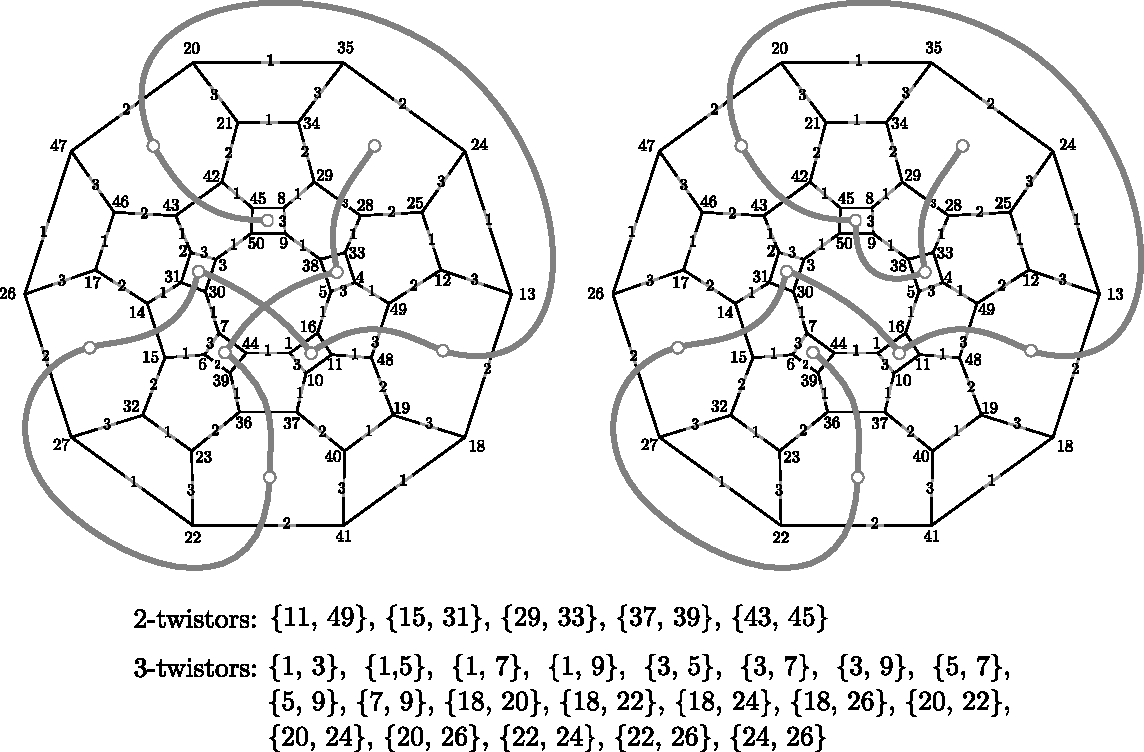
\includegraphics[width=14.5cm]{A.figs/resolutionDhip50A.pdf} \\
\caption{\sf This is a 50-vertex gem which behaves as the {\em attractor}.}
%(see \cite{lins1995gca})
%for the Weber-Seifert dodecahedral hyperbolic space.
%For a proof that it induces this space see also \cite{lins1995gca}.} 
\label{fig:resolutionDhip50A}
\end{center}
\end{figure}
%-----------------------------------

A crossing $x\in \mathbb{N}$ has 4 legs in counterclockwise 
order: $(4x-3, 4x-2, 4x-1, 4x)$.
A {\em duet} \index{duet} is a perfect matching of the legs.
The first entry of a \index{quintet} {\em quintet} is the number of the crossing.
Each crossing appears in two consecutive quintets. The second entry is $d$ 
or $u$ depending on whether the quintet holds the first or the second occurrence
of its crossing. The $d$ means that the southwest to the northeast passage
goes under, the $u$ means that it goes over. The third and fourth entries of a quintet
are legs and their order specifies a consistent orientation for all the components
of the link. The fifth and last entry of a quintet is the number of the component
of the link that contains the two legs. By properly embedding the quintets in the plane
and identifying the legs as specified by the duets we have a link diagram
with consistent orientation of all of its component. Thus to obtain a Gauss code
(\cite{rosenstiehl1976solution}, chapter 3 of \cite{Lins1980}, 
\cite{lins2008hsg}), for the link is straightforward. 
Even though 
there are 142 crossings in the projection, the number of 1-simplices
in the PL-link is only 68. This was obtained by a shortcutting technique 
which started with over two hundred 1-simplices:
each 0-simplex defines a triangle in $\mathbb{R}^3$; if this triangle
is not pierced by a 1-simplex, then the 0-simplex is removed from the link. 
Compare 68 with our theoretical 
bound, namely $12n^2=7500$, since $n=25$. We emphasize the issue that
the algorithm behaves very efficiently. 


\subsection{Duets of $DHIP_{50}^{142}$}
{\scriptsize
\begin{center}
$
\begin{array}{|c|c|c|c|c|c|c|c|} \hline
 1, 8 &
 2, 155 &
 3, 112 &
 4, 111 &
 5, 108 &
 6, 11 &
 7, 104 &
 9, 16 \\
 10, 101&
 12, 107&
 13, 564&
 14, 19&
 15, 102&
 17, 24&
 18, 97&
 20, 159 \\
 21, 158&
 22, 27&
 23, 468&
 25, 32&
 26, 465&
 28, 163&
 29, 340&
 30, 35 \\
 31, 336&
 33, 40&
 34, 267&
 36, 271&
 37, 560&
 38, 43&
 39, 268&
 41, 48 \\
 42, 75&
 44, 559&
 45, 72&
 46, 51&
 47, 76&
 49, 56&
 50, 495&
 52, 71 \\
 53, 68&
 54, 59&
 55, 188&
 57, 62&
 58, 185&
 60, 63&
 61, 500&
 64, 67 \\
 65, 70&
 66, 183&
 69, 184&
 73, 494&
 74, 79&
 77, 84&
 78, 263&
 80, 259 \\
 81, 258&
 82, 85&
 83, 26&
 86, 475&
 87, 92&
 88, 335&
 89, 472&
 90, 93 \\
 91, 466&
 94, 471&
 95, 98&
 96, 467&
 99, 156&
 100, 103&
 105, 110&
 106, 319 \\
 109, 320&
 113, 240&
 114, 239&
 115, 526&
 116, 117&
 118, 525&
 119, 122&
 120, 235 \\
 121, 236&
 123, 142&
 124, 127&
 125, 132&
 126, 531&
 128, 139&
 129, 136&
 130, 135 \\
 131, 532&
 133, 138&
 134, 317&
 137, 230&
 140, 141&
 143, 146&
 144, 231&
 145, 524 \\
 147, 528&
 148, 149&
 150, 527&
 151, 154&
 152, 383&
 153, 244&
 157, 164&
 160, 563 \\
 161, 464&
 162, 167&
 165, 172&
 166, 337&
 168, 463&
 169, 344&
 170, 175&
 171, 338 \\
 173, 180&
 174, 269&
 176, 275&
 177, 556&
 178, 181&
 179, 558&
 182, 497&
 186, 191 \\
 187, 496&
 189, 196&
 190, 489&
 192, 427&
 193, 432&
 194, 199&
 195, 488&
 197, 204 \\
 198, 435&
 200, 431&
 201, 448&
 202, 207&
 203, 544&
 205, 212&
 206, 443&
 208, 447 \\
 209, 446&
 210, 215&
 211, 538&
 213, 220&
 214, 483&
 216, 371&
 217, 370&
 218, 223 \\
 219, 376&
 221, 226&
 222, 373&
 224, 311&
 225, 522&
 227, 316&
 228, 229&
 232, 523 \\
 233, 530&
 234, 237&
 238, 529&
 241, 470&
 242, 247&
 243, 324&
 245, 252&
 246, 321 \\
 248, 327&
 249, 326&
 250, 253&
 251, 568&
 254, 329&
 255, 260&
 256, 479&
 257, 332 \\
 261, 334&
 262, 265&
 266, 333&
 270, 557&
 272, 339&
 273, 280&
 274, 553&
 276, 507 \\
 277, 506&
 278, 283&
 279, 416&
 281, 288&
 282, 413&
 284, 411&
 285, 552&
 286, 291 \\
 287, 504&
 289, 296&
 290, 295&
 292, 359&
 293, 364&
 294, 299&
 297, 304&
 298, 365 \\
 300, 363&
 301, 452&
 302, 305&
 303, 366&
 306, 451&
 307, 312&
 308, 369&
 309, 396 \\
 310, 313&
 314, 395&
 315, 318&
 322, 567&
 323, 392&
 325, 330&
 328, 473&
 331, 476 \\
 341, 404&
 342, 347&
 343, 408&
 345, 352&
 346, 511&
 348, 403&
 349, 516&
 350, 353 \\
 351, 512&
 354, 515&
 355, 360&
 356, 551&
 357, 514&
 358, 361&
 362, 519&
 367, 372 \\
 368, 445&
 374, 379&
 375, 484&
 377, 382&
 378, 535&
 380, 521&
 381, 536&
 384, 387 \\
 385, 390&
 386, 565&
 388, 391&
 389, 566&
 393, 456&
 394, 399&
 397, 402&
 398, 459 \\
 400, 455&
 401, 460&
 405, 510&
 406, 409&
 407, 508&
 410, 549&
 412, 505&
 414, 503 \\
 415, 420&
 417, 502&
 418, 421&
 419, 554&
 422, 501&
 423, 428&
 424, 499&
 425, 430 \\
 426, 429&
 433, 440&
 434, 485&
 436, 543&
 437, 542&
 438, 441&
 439, 546&
 442, 541 \\
 444, 537&
 449, 518&
 450, 453&
 454, 517&
 457, 462&
 458, 561&
 461, 562&
 469, 474 \\
 477, 482&
 478, 533&
 480, 539&
 481, 534&
 486, 545&
 487, 490&
 491, 548&
 492, 493 \\
 498, 555&
 509, 550&
 513, 520&
 540, 547 & & & & \\ \hline
\end{array}
$
\end{center}
}



%\subsection{Cylinders and framings}
%\begin{verbatim}
%boundary cylinder 1 linking number from 2-twistor {19,13} is -1
%boundary cylinder 2 linking number from 2-twistor {3,29} is 0
%boundary cylinder 3 linking number from 2-twistor {49,33} is -1
%boundary cylinder 4 linking number from 2-twistor {39,43} is -1
%boundary cylinder 5 linking number from 2-twistor {9,23} is -2
%boundary cylinder 6 linking number from 3-twistor {1,31} is 0
%boundary cylinder 7 linking number from 3-twistor {6,26} is 0
%boundary cylinder 8 linking number from 3-twistor {46,36} is 0
%boundary cylinder 9 linking number from 3-twistor {11,21} is 0
%\end{verbatim}


\subsection{Quintets, cylinders and framings of $DHIP_{50}^{142}$}


{\tiny
\begin{center}
$
\begin{array}{cccccc}
 \{1,\text{d},3,1,1\} & \{1,\text{u},4,2,3\} &
 \{2,\text{d},7,5,8\} & \{2,\text{u},8,6,1\} &
 \{3,\text{d},11,9,1\} & \{3,\text{u},10,12,1\} \\
 \{4,\text{d},13,15,8\} & \{4,\text{u},16,14,1\} &
 \{5,\text{d},18,20,2\} & \{5,\text{u},19,17,1\} &
 \{6,\text{d},24,22,1\} & \{6,\text{u},21,23,9\} \\
 \{7,\text{d},27,25,1\} & \{7,\text{u},28,26,5\} &
 \{8,\text{d},32,30,1\} & \{8,\text{u},31,29,4\} &
 \{9,\text{d},35,33,1\} & \{9,\text{u},34,36,3\} \\
 \{10,\text{d},39,37,9\} & \{10,\text{u},40,38,1\} &
 \{11,\text{d},42,44,8\} & \{11,\text{u},43,41,1\} &
 \{12,\text{d},48,46,1\} & \{12,\text{u},45,47,1\} \\
 \{13,\text{d},51,49,1\} & \{13,\text{u},50,52,6\} &
 \{14,\text{d},53,55,2\} & \{14,\text{u},56,54,1\} &
 \{15,\text{d},59,57,1\} & \{15,\text{u},60,58,8\} \\
 \{16,\text{d},61,63,8\} & \{16,\text{u},62,64,1\} &
 \{17,\text{d},66,68,2\} & \{17,\text{u},67,65,1\} &
 \{18,\text{d},70,72,1\} & \{18,\text{u},71,69,6\} \\
 \{19,\text{d},73,75,8\} & \{19,\text{u},76,74,1\} &
 \{20,\text{d},80,78,4\} & \{20,\text{u},79,77,1\} &
 \{21,\text{d},84,82,1\} & \{21,\text{u},81,83,3\} \\
 \{22,\text{d},86,88,9\} & \{22,\text{u},85,87,1\} &
 \{23,\text{d},91,89,9\} & \{23,\text{u},92,90,1\} &
 \{24,\text{d},93,95,1\} & \{24,\text{u},96,94,5\} \\
 \{25,\text{d},99,97,2\} & \{25,\text{u},98,100,1\} &
 \{26,\text{d},102,104,8\} & \{26,\text{u},103,101,1\} &
 \{27,\text{d},108,106,8\} & \{27,\text{u},107,105,1\} \\
 \{28,\text{d},109,111,3\} & \{28,\text{u},110,112,1\} &
 \{29,\text{d},115,113,6\} & \{29,\text{u},114,116,2\} &
 \{30,\text{d},120,118,8\} & \{30,\text{u},117,119,2\} \\
 \{31,\text{d},123,121,2\} & \{31,\text{u},122,124,2\} &
 \{32,\text{d},126,128,6\} & \{32,\text{u},127,125,2\} &
 \{33,\text{d},129,131,8\} & \{33,\text{u},132,130,2\} \\
 \{34,\text{d},135,133,2\} & \{34,\text{u},134,136,8\} &
 \{35,\text{d},138,140,2\} & \{35,\text{u},139,137,6\} &
 \{36,\text{d},141,143,2\} & \{36,\text{u},144,142,2\} \\
 \{37,\text{d},146,148,2\} & \{37,\text{u},145,147,6\} &
 \{38,\text{d},149,151,2\} & \{38,\text{u},150,152,8\} &
 \{39,\text{d},154,156,2\} & \{39,\text{u},155,153,3\} \\
 \{40,\text{d},159,157,2\} & \{40,\text{u},160,158,9\} &
 \{41,\text{d},164,162,2\} & \{41,\text{u},161,163,5\} &
 \{42,\text{d},167,165,2\} & \{42,\text{u},166,168,8\} \\
 \{43,\text{d},172,170,2\} & \{43,\text{u},171,169,4\} &
 \{44,\text{d},175,173,2\} & \{44,\text{u},174,176,3\} &
 \{45,\text{d},179,177,9\} & \{45,\text{u},180,178,2\} \\
 \{46,\text{d},181,183,2\} & \{46,\text{u},184,182,6\} &
 \{47,\text{d},188,186,2\} & \{47,\text{u},185,187,8\} &
 \{48,\text{d},192,190,7\} & \{48,\text{u},191,189,2\} \\
 \{49,\text{d},196,194,2\} & \{49,\text{u},195,193,7\} &
 \{50,\text{d},200,198,5\} & \{50,\text{u},199,197,2\} &
 \{51,\text{d},204,202,2\} & \{51,\text{u},203,201,7\} \\
 \{52,\text{d},207,205,2\} & \{52,\text{u},206,208,5\} &
 \{53,\text{d},209,211,7\} & \{53,\text{u},212,210,2\} &
 \{54,\text{d},214,216,8\} & \{54,\text{u},215,213,2\} \\
 \{55,\text{d},217,219,4\} & \{55,\text{u},220,218,2\} &
 \{56,\text{d},222,224,5\} & \{56,\text{u},223,221,2\} &
 \{57,\text{d},226,228,2\} & \{57,\text{u},227,225,6\} \\
 \{58,\text{d},230,232,6\} & \{58,\text{u},229,231,2\} &
 \{59,\text{d},233,235,8\} & \{59,\text{u},236,234,2\} &
 \{60,\text{d},237,239,2\} & \{60,\text{u},240,238,6\} \\
 \{61,\text{d},244,242,3\} & \{61,\text{u},241,243,9\} &
 \{62,\text{d},247,245,3\} & \{62,\text{u},246,248,4\} &
 \{63,\text{d},251,249,9\} & \{63,\text{u},252,250,3\} \\
 \{64,\text{d},253,255,3\} & \{64,\text{u},254,256,5\} &
 \{65,\text{d},257,259,4\} & \{65,\text{u},260,258,3\} &
 \{66,\text{d},263,261,4\} & \{66,\text{u},264,262,3\} \\
 \{67,\text{d},266,268,9\} & \{67,\text{u},265,267,3\} &
 \{68,\text{d},270,272,8\} & \{68,\text{u},271,269,3\} &
 \{69,\text{d},276,274,8\} & \{69,\text{u},275,273,3\} \\
 \{70,\text{d},279,277,6\} & \{70,\text{u},280,278,3\} &
 \{71,\text{d},284,282,5\} & \{71,\text{u},283,281,3\} &
 \{72,\text{d},287,285,9\} & \{72,\text{u},288,286,3\} \\
 \{73,\text{d},292,290,6\} & \{73,\text{u},291,289,3\} &
 \{74,\text{d},296,294,3\} & \{74,\text{u},295,293,6\} &
 \{75,\text{d},299,297,3\} & \{75,\text{u},300,298,4\} \\
 \{76,\text{d},304,302,3\} & \{76,\text{u},303,301,5\} &
 \{77,\text{d},305,307,3\} & \{77,\text{u},308,306,8\} &
 \{78,\text{d},312,310,3\} & \{78,\text{u},311,309,5\} \\
 \{79,\text{d},313,315,3\} & \{79,\text{u},314,316,6\} &
 \{80,\text{d},319,317,8\} & \{80,\text{u},318,320,3\} &
 \{81,\text{d},324,322,9\} & \{81,\text{u},323,321,4\} \\
 \{82,\text{d},326,328,9\} & \{82,\text{u},327,325,4\} &
 \{83,\text{d},330,332,4\} & \{83,\text{u},331,329,5\} &
 \{84,\text{d},335,333,9\} & \{84,\text{u},334,336,4\} \\
 \{85,\text{d},339,337,8\} & \{85,\text{u},340,338,4\} &
 \{86,\text{d},344,342,4\} & \{86,\text{u},341,343,5\} &
 \{87,\text{d},347,345,4\} & \{87,\text{u},346,348,9\} \\
 \{88,\text{d},351,349,6\} & \{88,\text{u},352,350,4\} &
 \{89,\text{d},353,355,4\} & \{89,\text{u},354,356,8\} &
 \{90,\text{d},357,359,6\} & \{90,\text{u},360,358,4\} \\
 \{91,\text{d},364,362,6\} & \{91,\text{u},361,363,4\} &
 \{92,\text{d},365,367,4\} & \{92,\text{u},368,366,5\} &
 \{93,\text{d},372,370,4\} & \{93,\text{u},371,369,8\} \\
 \{94,\text{d},376,374,4\} & \{94,\text{u},375,373,5\} &
 \{95,\text{d},379,377,4\} & \{95,\text{u},380,378,6\} &
 \{96,\text{d},382,384,4\} & \{96,\text{u},383,381,8\} \\
 \{97,\text{d},387,385,4\} & \{97,\text{u},386,388,9\} &
 \{98,\text{d},391,389,9\} & \{98,\text{u},390,392,4\} &
 \{99,\text{d},393,395,6\} & \{99,\text{u},396,394,5\} \\
 \{100,\text{d},399,397,5\} & \{100,\text{u},400,398,5\} &
 \{101,\text{d},403,401,9\} & \{101,\text{u},402,404,5\} &
 \{102,\text{d},407,405,6\} & \{102,\text{u},408,406,5\} \\
 \{103,\text{d},410,412,8\} & \{103,\text{u},409,411,5\} &
 \{104,\text{d},414,416,6\} & \{104,\text{u},413,415,5\} &
 \{105,\text{d},419,417,9\} & \{105,\text{u},420,418,5\} \\
 \{106,\text{d},421,423,5\} & \{106,\text{u},424,422,6\} &
 \{107,\text{d},425,427,7\} & \{107,\text{u},428,426,5\} &
 \{108,\text{d},429,431,5\} & \{108,\text{u},432,430,7\} \\
 \{109,\text{d},435,433,5\} & \{109,\text{u},436,434,6\} &
 \{110,\text{d},439,437,7\} & \{110,\text{u},440,438,5\} &
 \{111,\text{d},441,443,5\} & \{111,\text{u},444,442,6\} \\
 \{112,\text{d},448,446,7\} & \{112,\text{u},447,445,5\} &
 \{113,\text{d},451,449,8\} & \{113,\text{u},452,450,5\} &
 \{114,\text{d},454,456,6\} & \{114,\text{u},453,455,5\} \\
 \{115,\text{d},460,458,9\} & \{115,\text{u},459,457,5\} &
 \{116,\text{d},463,461,8\} & \{116,\text{u},462,464,5\} &
 \{117,\text{d},468,466,9\} & \{117,\text{u},465,467,5\} \\
 \{118,\text{d},472,470,9\} & \{118,\text{u},471,469,5\} &
 \{119,\text{d},473,475,9\} & \{119,\text{u},474,476,5\} &
 \{120,\text{d},479,477,5\} & \{120,\text{u},478,480,6\} \\
 \{121,\text{d},482,484,5\} & \{121,\text{u},481,483,8\} &
 \{122,\text{d},486,488,7\} & \{122,\text{u},485,487,6\} &
 \{123,\text{d},489,491,7\} & \{123,\text{u},490,492,6\} \\
 \{124,\text{d},496,494,8\} & \{124,\text{u},493,495,6\} &
 \{125,\text{d},498,500,8\} & \{125,\text{u},497,499,6\} &
 \{126,\text{d},501,503,6\} & \{126,\text{u},502,504,9\} \\
 \{127,\text{d},506,508,6\} & \{127,\text{u},505,507,8\} &
 \{128,\text{d},510,512,6\} & \{128,\text{u},509,511,9\} &
 \{129,\text{d},516,514,6\} & \{129,\text{u},513,515,8\} \\
 \{130,\text{d},519,517,6\} & \{130,\text{u},518,520,8\} &
 \{131,\text{d},523,521,6\} & \{131,\text{u},522,524,6\} &
 \{132,\text{d},525,527,8\} & \{132,\text{u},528,526,6\} \\
 \{133,\text{d},532,530,8\} & \{133,\text{u},529,531,6\} &
 \{134,\text{d},536,534,8\} & \{134,\text{u},535,533,6\} &
 \{135,\text{d},538,540,7\} & \{135,\text{u},539,537,6\} \\
 \{136,\text{d},542,544,7\} & \{136,\text{u},541,543,6\} &
 \{137,\text{d},548,546,7\} & \{137,\text{u},547,545,7\} &
 \{138,\text{d},551,549,8\} & \{138,\text{u},552,550,9\} \\
 \{139,\text{d},556,554,9\} & \{139,\text{u},553,555,8\} &
 \{140,\text{d},560,558,9\} & \{140,\text{u},559,557,8\} &
 \{141,\text{d},562,564,8\} & \{141,\text{u},561,563,9\} \\
 \{142,\text{d},566,568,9\} & \{142,\text{u},567,565,9\} &
\end{array}
$
\end{center}
}

\begin{figure}[!htb]
\begin{center}
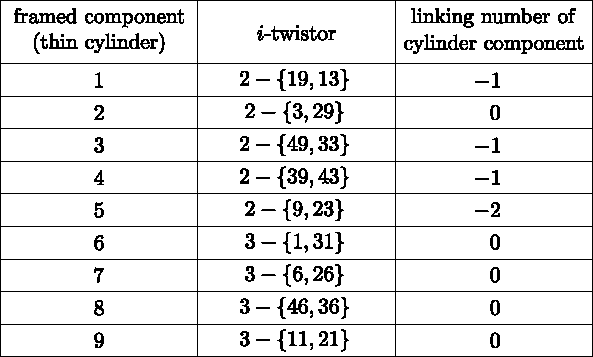
\includegraphics[width=5.8cm]{A.figs/U2.pdf}
\end{center}
\end{figure}


\section*{Appendix B: all figures for the $r_5^{24}$-example. This produces
an overview of the data structure and their interrelations illustrating the general case
of the algorithm}

In the following figures, the notation
% $\nabla_{v,1}$ denotes the PL3-face dual of the vertex $v$ in $E\mathcal{H}_1^\star$.
 $\nabla_{v,i+1}$, $i\geq1$, denotes the PL3-face dual of the
vertex $v$ of the input gem obtained after the $i$-th $bp$-move is performed. If after the $i$-th
$bp$-move $\nabla_{v,i}$ does not change, then $\nabla_{v,i+1}=\nabla_{v,i}$. When there is a change,
it is an $\epsilon$-change.


%-----------------------------------
\begin{figure}[!htb]
\begin{center}
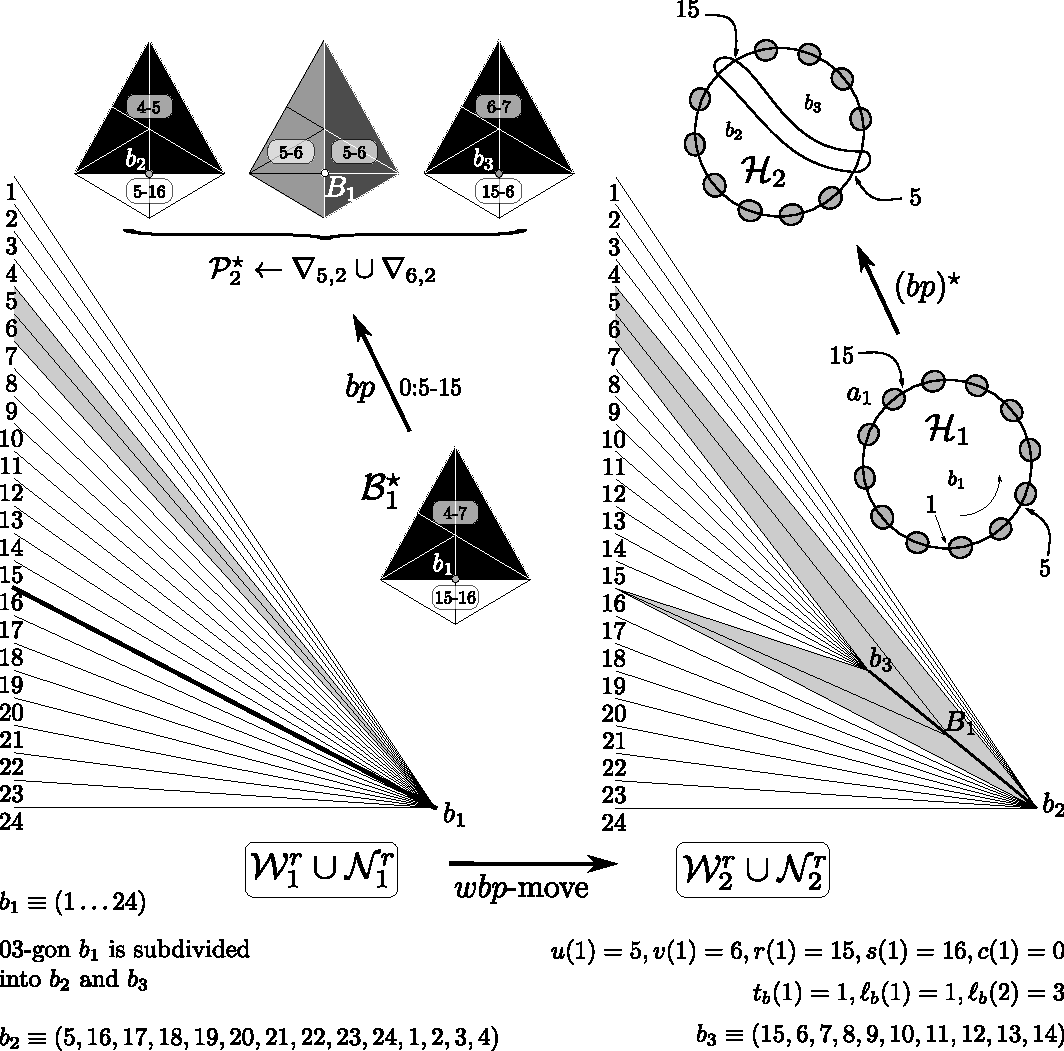
\includegraphics[width=15cm]{A.figs/bpandwinglist01.pdf} \\
\caption{\sf 
$\mathcal{H}^\star_{2} \leftarrow \mathcal{H}^\star_1 
\cup (\mathcal{P}_{2}^\star \backslash \mathcal{B}_1^\star)$. 
Pillow $\mathcal{P}_{2}^\star \leftarrow 
\nabla_{5,12}\cup \nabla_{6,12}$
($r^{24}_5$-example).}
\label{fig:winglist01}
\end{center}
\end{figure}
%-----------------------------------

%-----------------------------------
\begin{figure}
\begin{center}
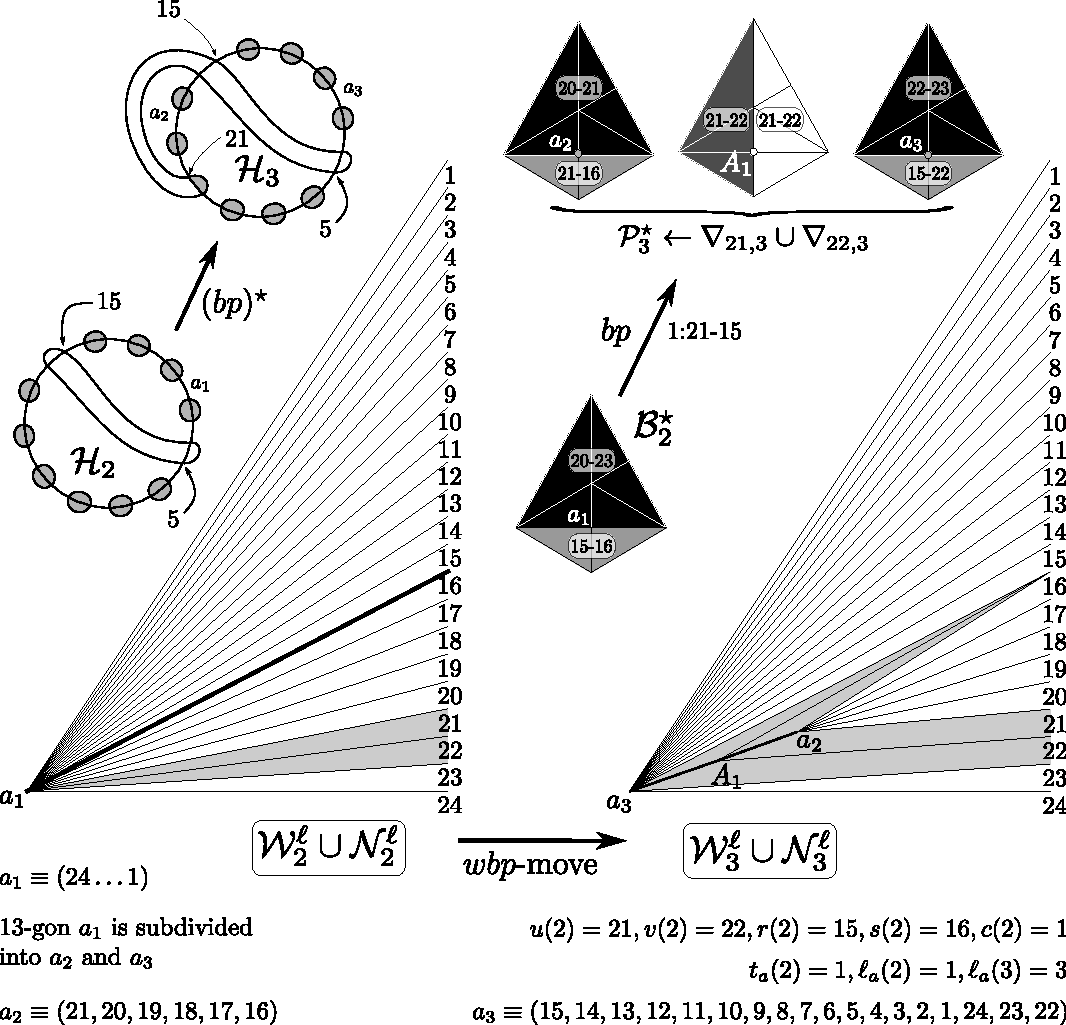
\includegraphics[width=15cm]{A.figs/bpandwinglist02.pdf} \\
\caption{\sf 
$\mathcal{H}^\star_{3} \leftarrow \mathcal{H}^\star_2 
\cup (\mathcal{P}_{3}^\star \backslash \mathcal{B}_2^\star)$. 
Pillow $\mathcal{P}_{3}^\star \leftarrow 
\nabla_{21,12}\cup \nabla_{22,12}$
($r^{24}_5$-example).}
\label{fig:winglist02}
\end{center}
\end{figure}
%-----------------------------------

%-----------------------------------
\begin{figure}
\begin{center}
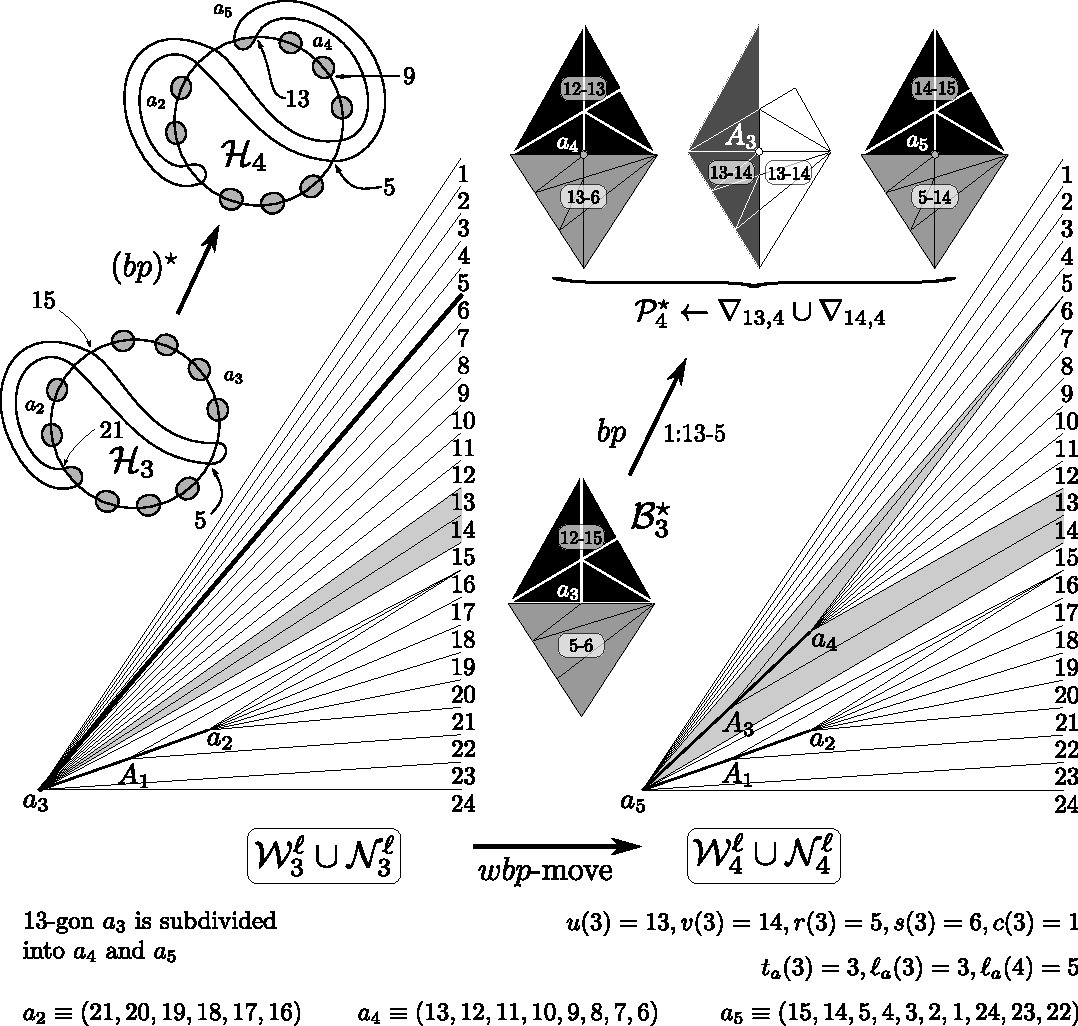
\includegraphics[width=15cm]{A.figs/bpandwinglist03.pdf} \\
\caption{\sf 
$\mathcal{H}^\star_{4} \leftarrow \mathcal{H}^\star_3 
\cup (\mathcal{P}_{4}^\star \backslash \mathcal{B}_3^\star)$. 
Pillow $\mathcal{P}_{4}^\star \leftarrow 
\nabla_{13,12}\cup \nabla_{14,12}$
($r^{24}_5$-example).}
\label{fig:winglist03}
\end{center}
\end{figure}
%-----------------------------------

%-----------------------------------
\begin{figure}
\begin{center}
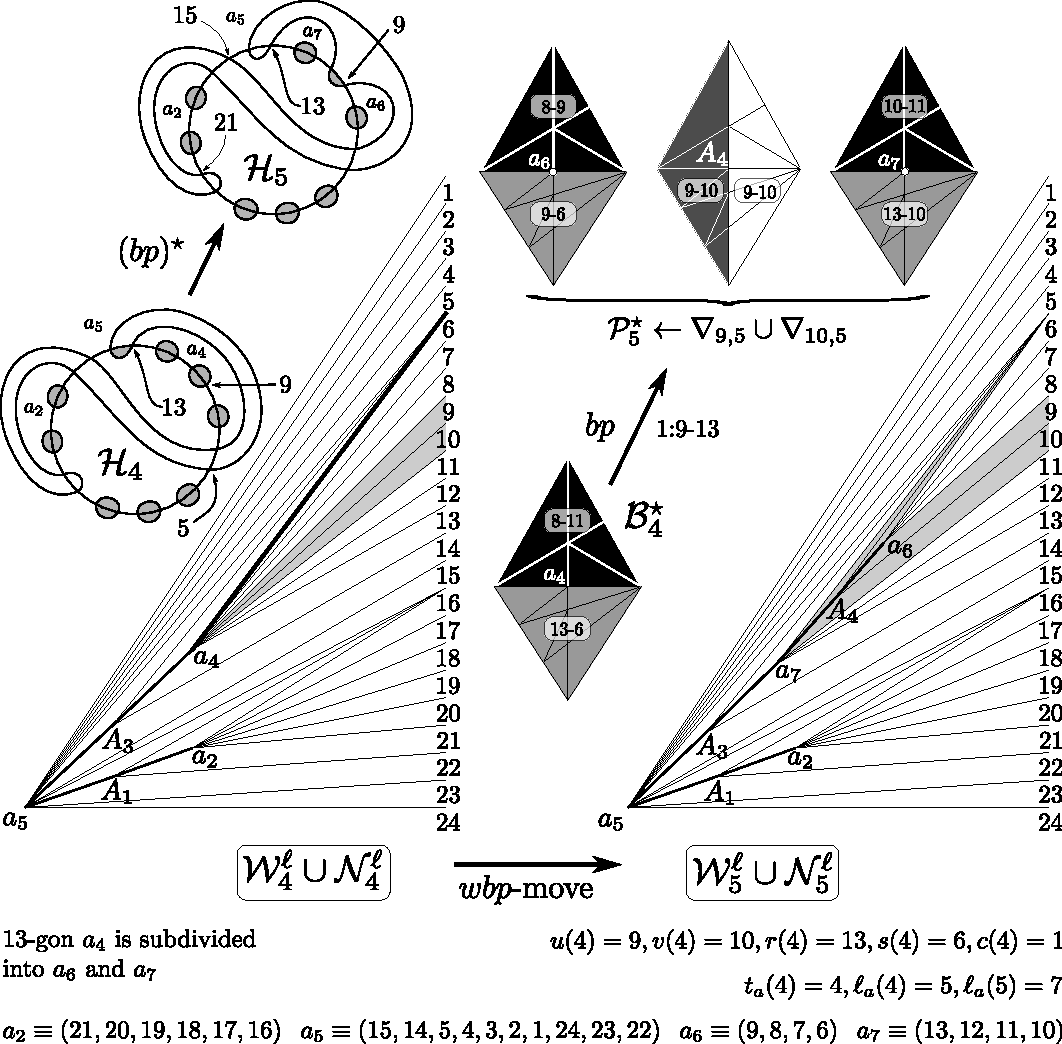
\includegraphics[width=15cm]{A.figs/bpandwinglist04.pdf} \\
\caption{\sf 
$\mathcal{H}^\star_{5} \leftarrow \mathcal{H}^\star_4 
\cup (\mathcal{P}_{5}^\star \backslash \mathcal{B}_4^\star)$. 
Pillow $\mathcal{P}_{5}^\star \leftarrow 
\nabla_{9,12}\cup \nabla_{10,12}$
($r^{24}_5$-example).}
\label{fig:winglist04}
\end{center}
\end{figure}
%-----------------------------------

%-----------------------------------
\begin{figure}
\begin{center}
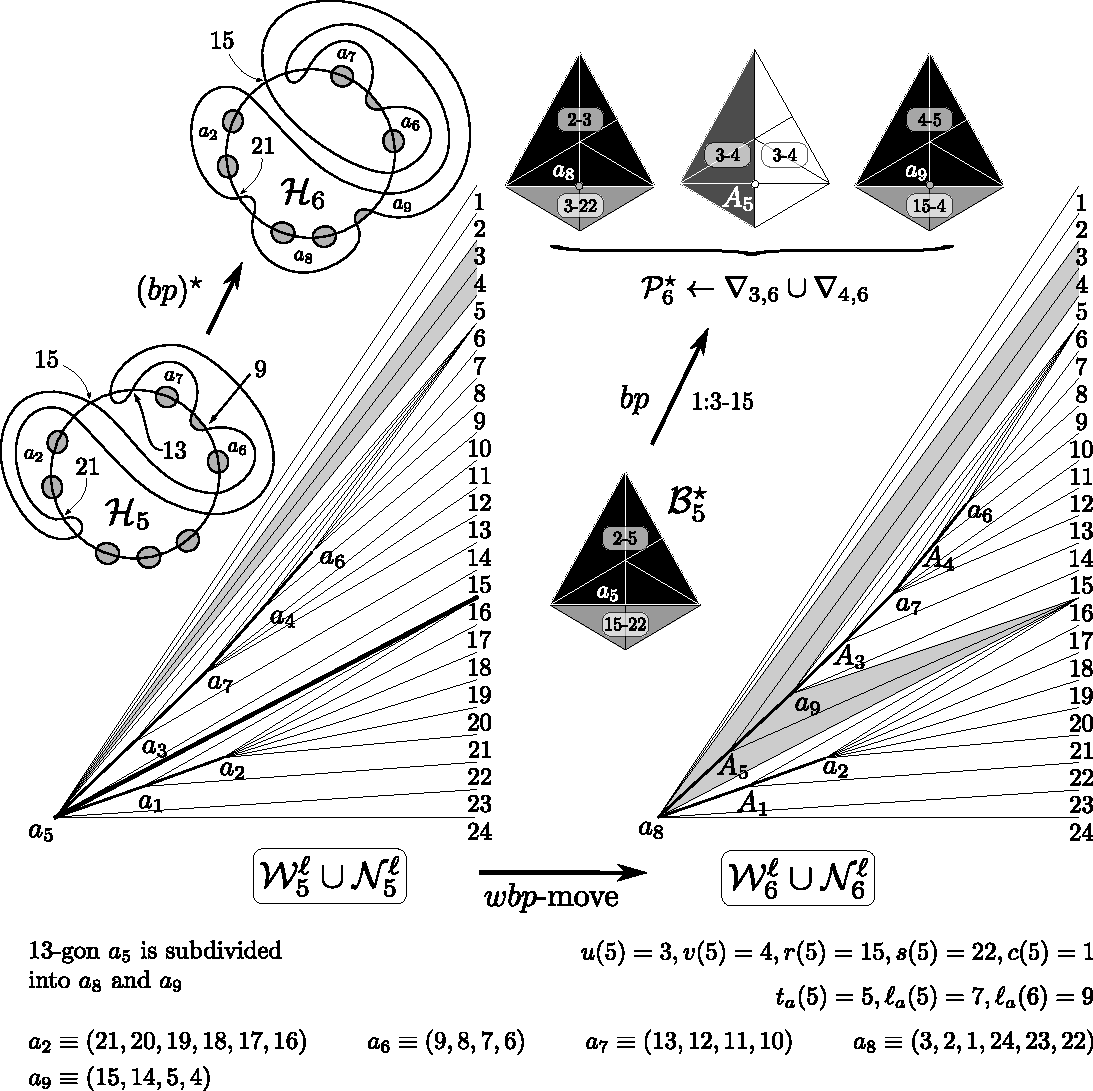
\includegraphics[width=15cm]{A.figs/bpandwinglist05.pdf} \\
\caption{\sf 
$\mathcal{H}^\star_{6} \leftarrow \mathcal{H}^\star_5 
\cup (\mathcal{P}_{6}^\star \backslash \mathcal{B}_5^\star)$. 
Pillow $\mathcal{P}_{6}^\star \leftarrow 
\nabla_{3,12}\cup \nabla_{4,12}$
($r^{24}_5$-example).}
\label{fig:winglist05}
\end{center}
\end{figure}
%-----------------------------------

%-----------------------------------
\begin{figure}
\begin{center}
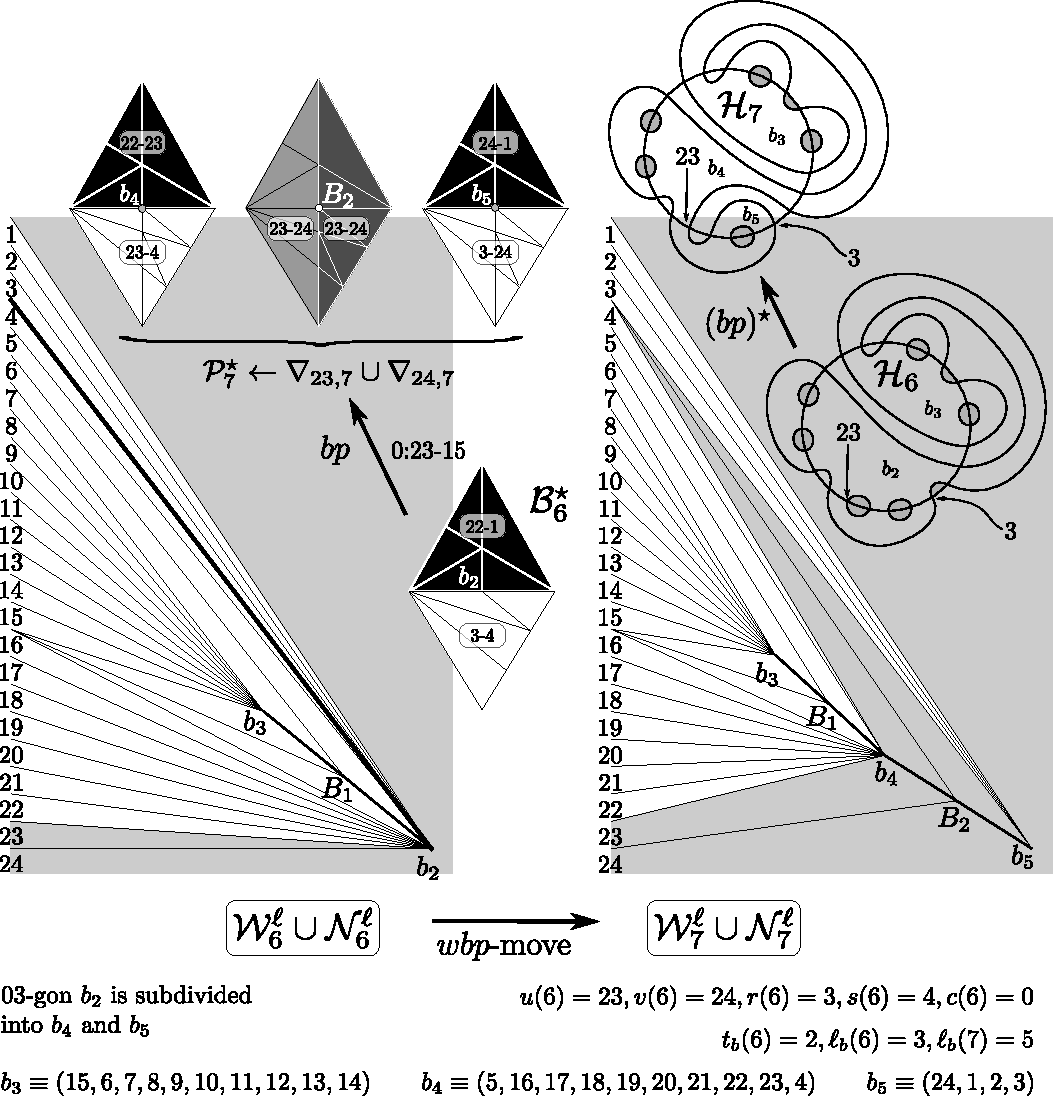
\includegraphics[width=15cm]{A.figs/bpandwinglist06.pdf} \\
\caption{\sf 
$\mathcal{H}^\star_{7} \leftarrow \mathcal{H}^\star_6 
\cup (\mathcal{P}_{7}^\star \backslash \mathcal{B}_6^\star)$. 
Pillow $\mathcal{P}_{7}^\star \leftarrow 
\nabla_{23,12}\cup \nabla_{24,12}$
($r^{24}_5$-example).}
\label{fig:winglist06}
\end{center}
\end{figure}
%-----------------------------------


%-----------------------------------
\begin{figure}
\begin{center}
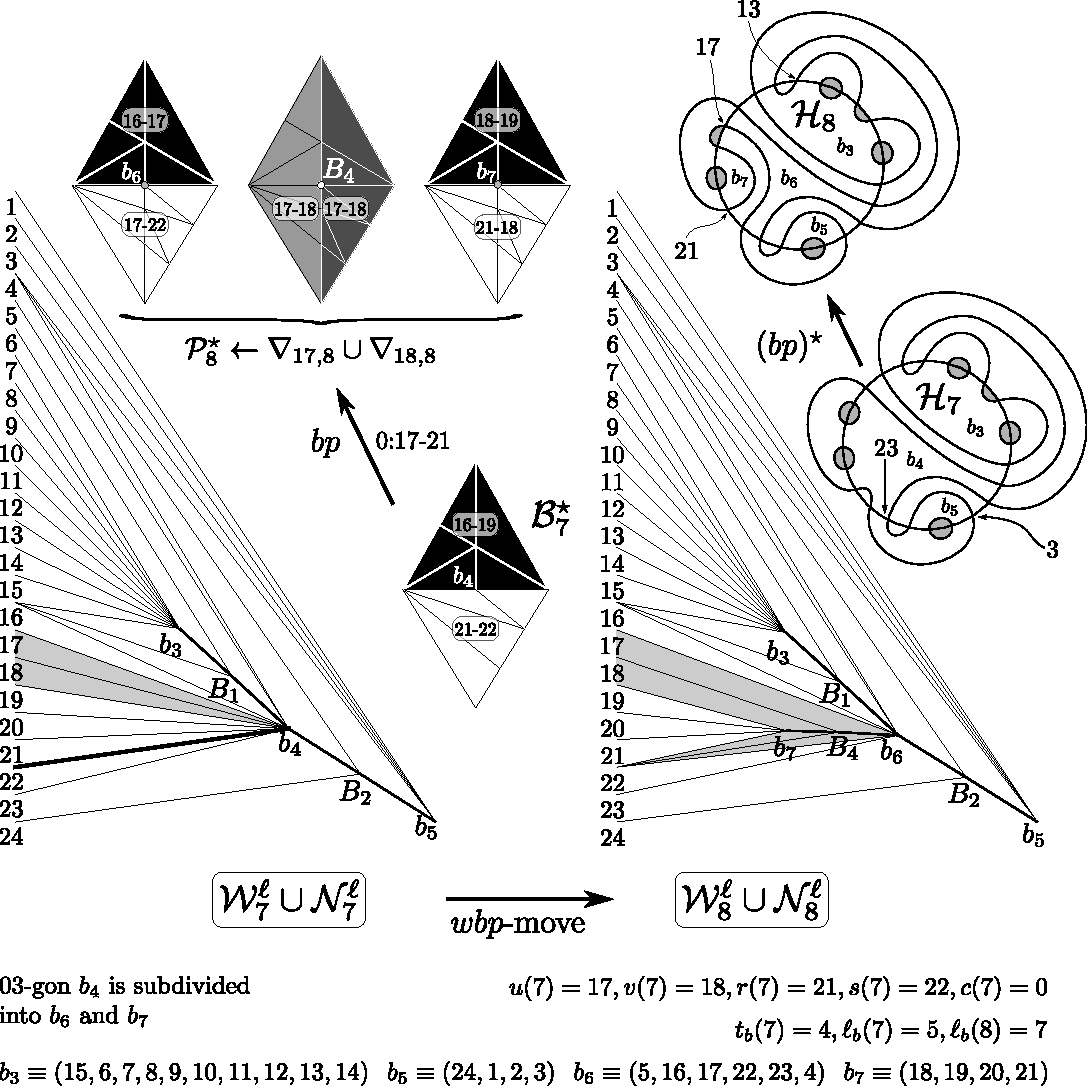
\includegraphics[width=15cm]{A.figs/bpandwinglist07.pdf} \\
\caption{\sf 
$\mathcal{H}^\star_{8} \leftarrow \mathcal{H}^\star_7 
\cup (\mathcal{P}_{8}^\star \backslash \mathcal{B}_7^\star)$. 
Pillow $\mathcal{P}_{8}^\star \leftarrow 
\nabla_{17,12}\cup \nabla_{18,12}$
($r^{24}_5$-example).}
\label{fig:winglist07}
\end{center}
\end{figure}
%-----------------------------------

%-----------------------------------
\begin{figure}
\begin{center}
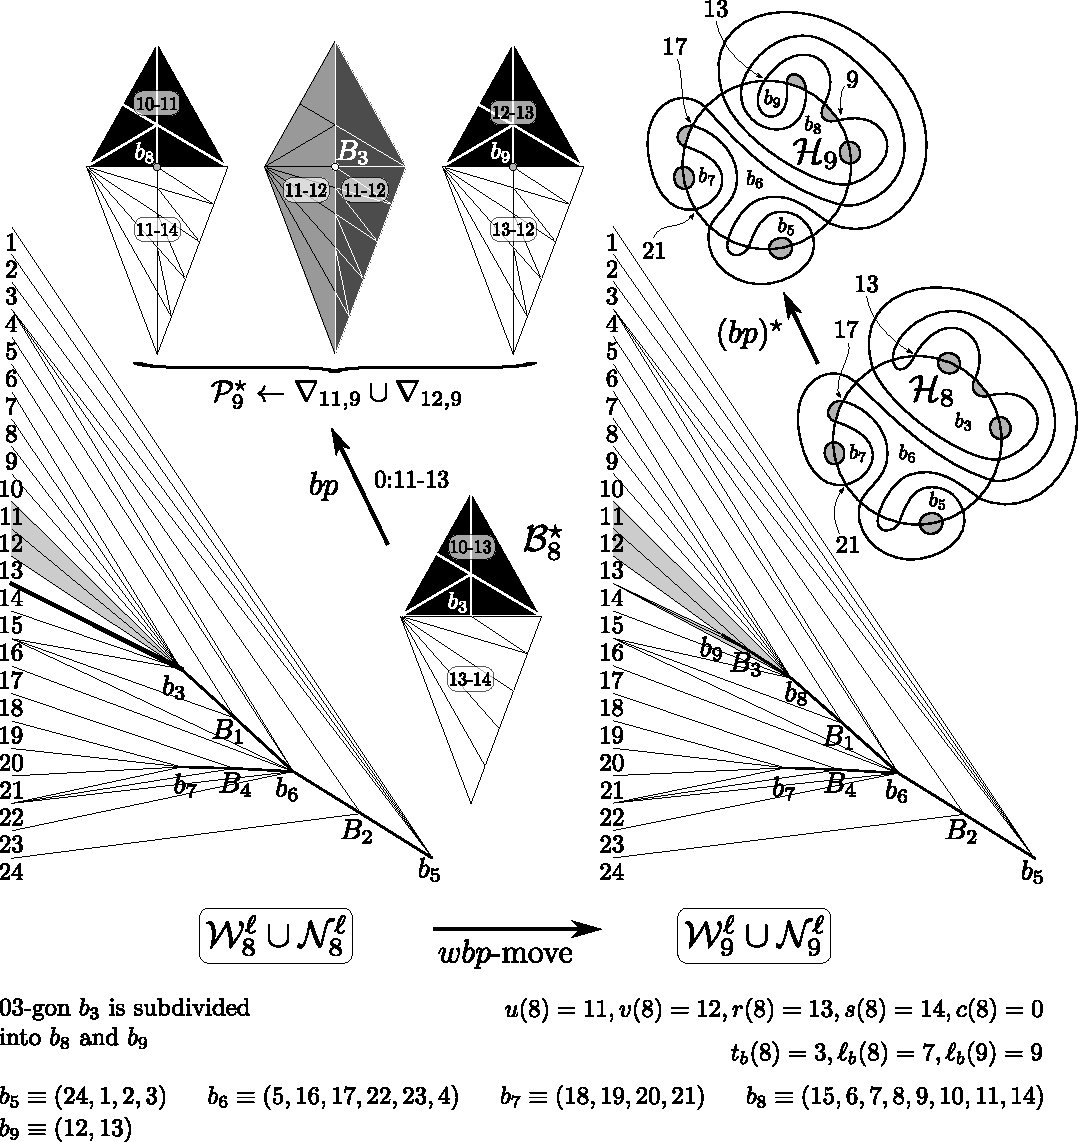
\includegraphics[width=15cm]{A.figs/bpandwinglist08.pdf} \\
\caption{\sf 
$\mathcal{H}^\star_{9} \leftarrow \mathcal{H}^\star_8 
\cup (\mathcal{P}_{9}^\star \backslash \mathcal{B}_8^\star)$. 
Pillow $\mathcal{P}_{9}^\star \leftarrow 
\nabla_{11,12}\cup \nabla_{12,12}$
($r^{24}_5$-example).}
\label{fig:winglist08}
\end{center}
\end{figure}
%-----------------------------------

%-----------------------------------
\begin{figure}
\begin{center}
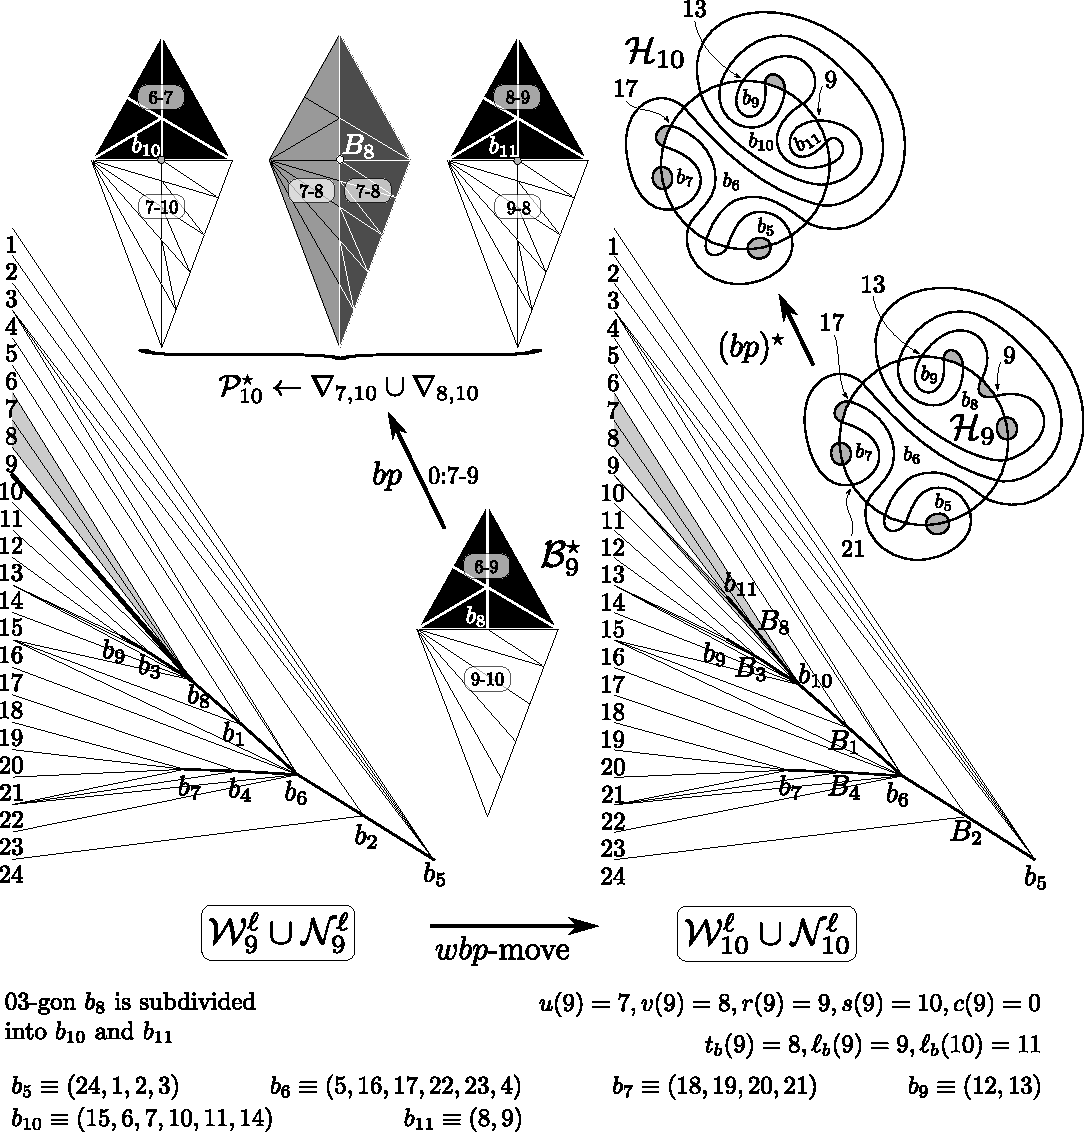
\includegraphics[width=15cm]{A.figs/bpandwinglist09.pdf} \\
\caption{\sf 
$\mathcal{H}^\star_{10} \leftarrow \mathcal{H}^\star_9 
\cup (\mathcal{P}_{10}^\star \backslash \mathcal{B}_9^\star)$. 
Pillow $\mathcal{P}_{10}^\star \leftarrow 
\nabla_{7,12}\cup \nabla_{8,12}$
($r^{24}_5$-example).}
\label{fig:winglist09}
\end{center}
\end{figure}
%-----------------------------------

%-----------------------------------
\begin{figure}
\begin{center}
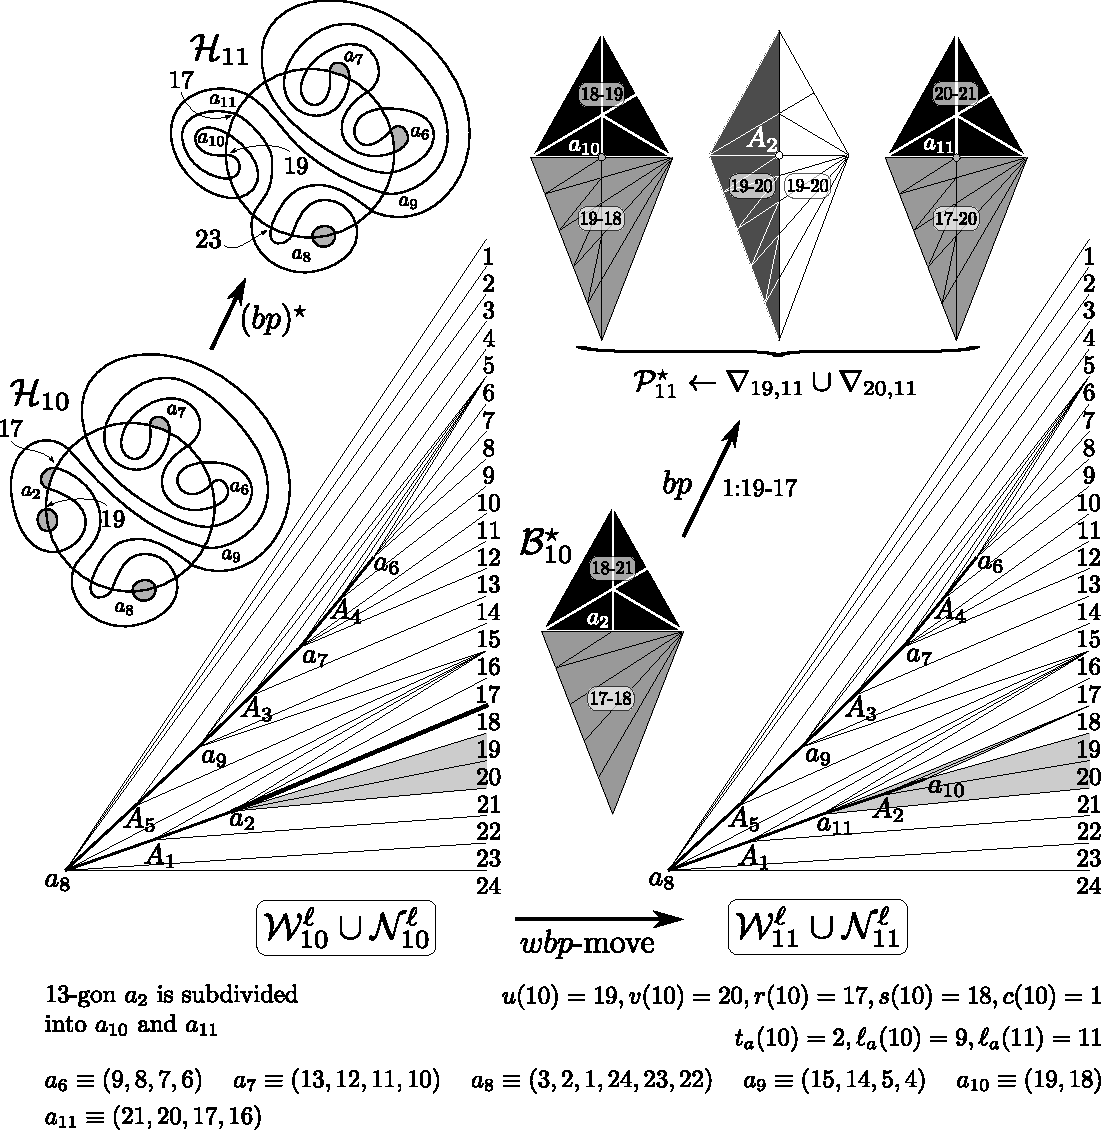
\includegraphics[width=15cm]{A.figs/bpandwinglist10.pdf} \\
\caption{\sf 
$\mathcal{H}^\star_{11} \leftarrow \mathcal{H}^\star_{10}
\cup (\mathcal{P}_{11}^\star \backslash \mathcal{B}_{10}^\star)$.
Pillow $\mathcal{P}_{11}^\star \leftarrow 
\nabla_{19,12}\cup \nabla_{20,12}$
($r^{24}_5$-example).}
\label{fig:winglist10}
\end{center}
\end{figure}
%-----------------------------------

%-----------------------------------
\begin{figure}
\begin{center}
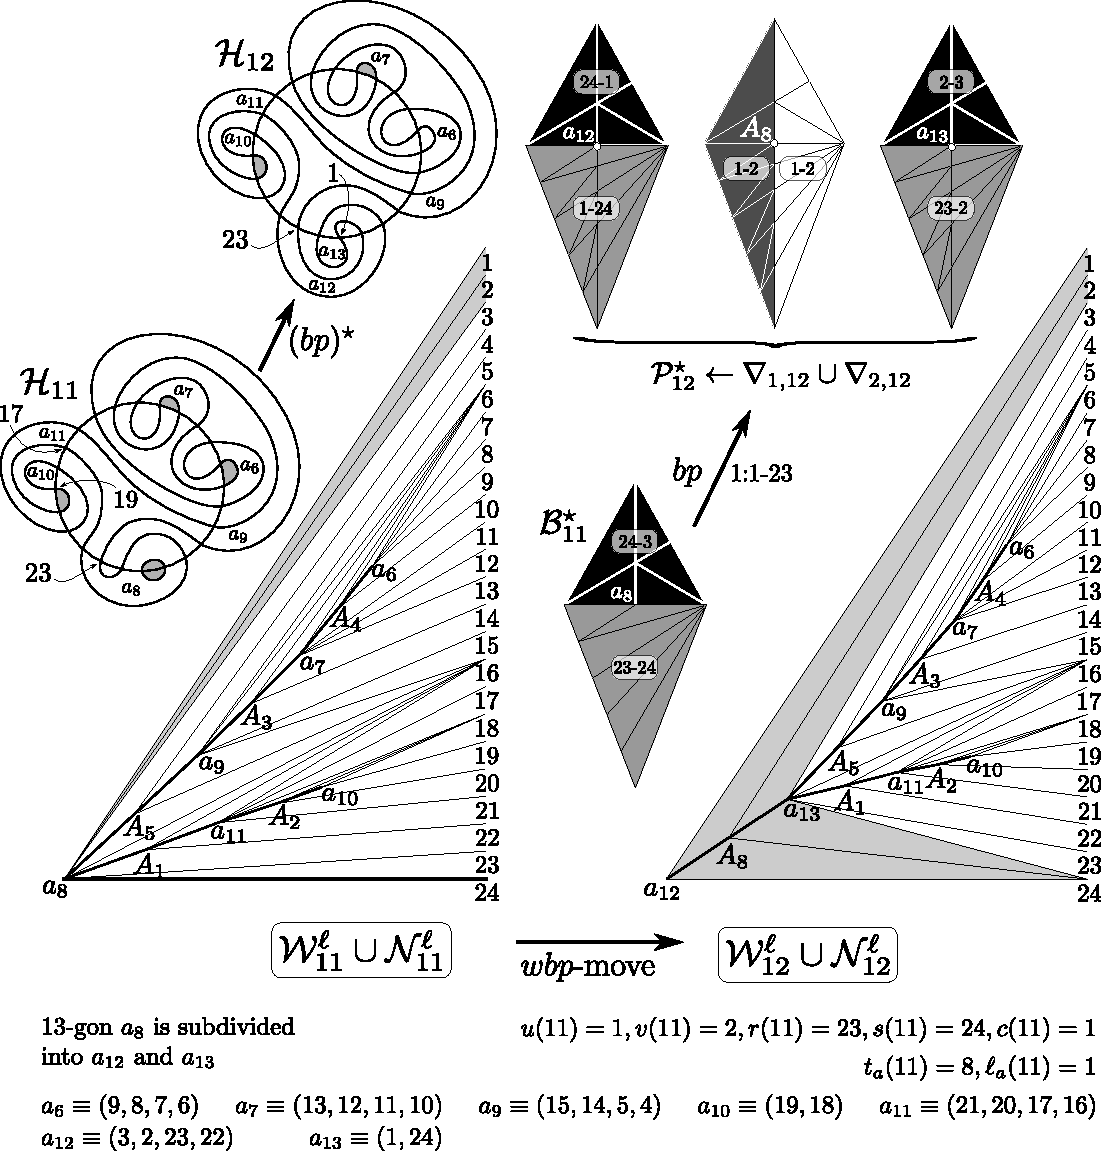
\includegraphics[width=15cm]{A.figs/bpandwinglist11.pdf} \\
\caption{\sf 
$\mathcal{H}^\star_{12} \leftarrow \mathcal{H}^\star_{11} 
\cup (\mathcal{P}_{12}^\star \backslash \mathcal{B}_{11}^\star)$. 
Pillow $\mathcal{P}_{12}^\star \leftarrow \nabla_{1,12}\cup \nabla_{2,12}$
($r^{24}_5$-example).}
\label{fig:winglist11}
\end{center}
\end{figure}
%-----------------------------------

%-----------------------------------
%\begin{figure}
%\begin{center}
%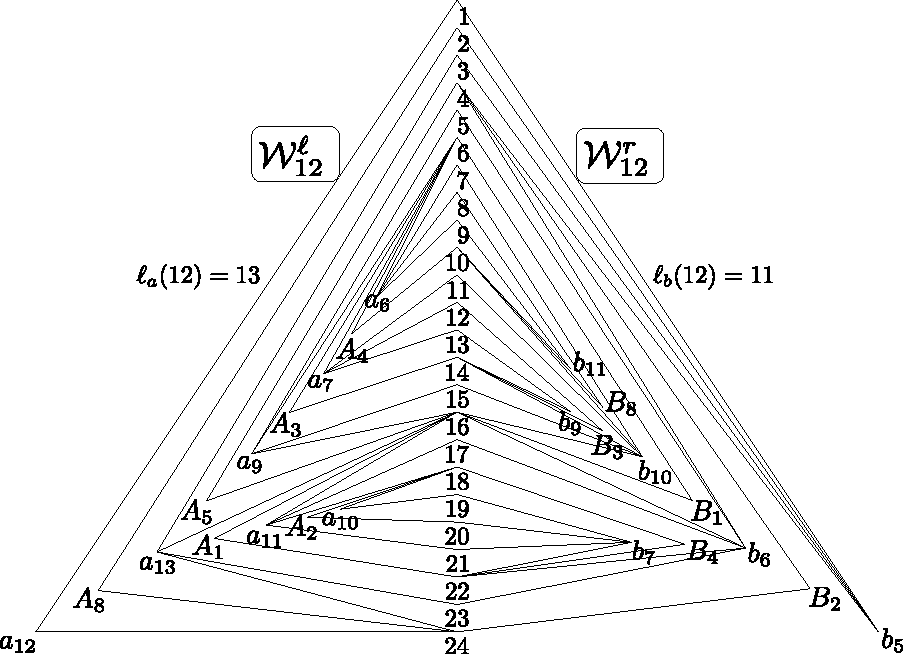
\includegraphics[width=15cm]{A.figs/bpandwinglist12.pdf} \\
%\caption{\sf 
%$\mathcal{H}^\star_{12} \leftarrow \mathcal{H}^\star_{11} 
%\cup (\mathcal{P}_{12}^\star \backslash \mathcal{B}_{11}^\star)$ 
%and wings (without nervures) of $\mathcal{H}^\star_{12}$
%($r^{24}_5$-example).}
%\label{fig:winglist12}
%\end{center}
%\end{figure}



%-----------------------------------
%\bibliographystyle{plain}
%\bibliographystyle{is-alpha}
%\addcontentsline{toc}{bibliografia}{\MakeTextUppercase{Refer�ncias Bibliogr�ficas}}
%\bibliography{d:/slsl\3.DadosSostenes.35.ArtigosLivros.bibtexGoogleScholar/bibtexIndex.bib} % bib file is slsl.bib
%\bibliography{~/home/ricardo/Dropbox/35.ArtigosLivros.bibtexGoogleScholar/bibtexIndex.bib}
%\bibliography{bibtexIndex.bib}
%\bibliography{slsl}

% \vspace{10mm}
% \begin{center}
% 
% 
% \hspace{7mm}
% \begin{tabular}{l}
%    S\'ostenes L. Lins\\
%    Centro de Inform\'atica, UFPE \\
%    Recife--PE \\
%    Brazil\\
%    sostenes@cin.ufpe.br
% \end{tabular}
% \hspace{20mm}
% \begin{tabular}{l}
%    Ricardo N. Machado\\
%    N�cleo de Forma��o de Docentes, UFPE\\
%    Caruaru--PE \\
%    Brazil\\
%    ricardonmachado@gmail.com
% \end{tabular}
% 
% \end{center}


%\end{document}



